\documentclass[10pt]{beamer}

\usepackage[utf8]{inputenc}
\usepackage{tcolorbox}
\usepackage{tikz}
\usepackage{tikz-3dplot}
\usetikzlibrary{intersections,calc,,angles,quotes,through}
\usepackage{amsmath}
\usepackage{graphicx}
\usepackage{cases}
\def \heart {\textcolor{blue}{$\heartsuit$} }
\def \C {\mathcal{C}}
\def \orthog {\underline{\perp}}
\def\arcos{\operatorname{arcos}}
\def \deg {^{\circ}}

\newcommand{\vect}[1] {
  \overrightarrow{#1}}

\tcbset{%
	basic/.style={colframe=black,
		      colback=white,
		      top= 0mm,
		      bottom = 2mm,
		      boxsep=0mm
		      }
}
\tikzset{
    invisible/.style={opacity=0},
    visible on/.style={alt={#1{}{invisible}}},
    alt/.code args={<#1>#2#3}{%
      \alt<#1>{\pgfkeysalso{#2}}{\pgfkeysalso{#3}} % \pgfkeysalso doesn't change the path
    },
  }

    
\begin{document}  
    \beamertemplatenavigationsymbolsempty
    \setlength{\abovedisplayskip}{0pt}
    \setlength{\belowdisplayskip}{0pt}
    \frame{
	  
	  \frametitle{Q2 Septembre 2002.}
	  \renewcommand{\theenumi}{\alph{enumi})}
	  Dans le plan muni d’un repère orthonormé $Oxy$, on considère les points
	  $A(0, a)$, $B(b, 0)$ et $C(-b, 0)$ formant un triangle isocèle $(a, b > 0)$. On considère
	  un point $P (\lambda, 0)$ variable sur $Ox$.
	  \begin{enumerate}
	   \item Quelles sont les coordonnées des pieds $B'$ et $C'$ des perpendiculaires abaissées
		 de $P$ sur $AB$ et $AC$ respectivement.
	   \item Quel est le lieu du milieu de $[B',C']$ lorsque $P$ parcourt le segment $[B,C]$ ?
	   \item Quelle est l’équation de la droite $d$ perpendiculaire à $B'C'$ menée par $P$ ?
		 Montrer qu’elle passe par un point fixe quand $P$ parcourt l’axe $0x$.
	  \end{enumerate}

	  \vfill
	  
	  \pause
	  
	   \begin{tcolorbox}[basic] \smallskip
	     \centering\underline{Procédé} \smallskip
	     \begin{columns}[c]
	     \column{.333\textwidth}\centering 
	     \vspace{-1mm}
	     \renewcommand{\theenumi}{\alph{enumi})}
	     \begin{enumerate}
	      \item $B'\equiv BB' \bot B'P$, \\ \smallskip
		    $C'\equiv CC' \bot C'P$. 
	     \end{enumerate}
	     
	     \column{.34\textwidth}\centering
	     \begin{enumerate}
	      \item[b).] $M(\lambda)=\dfrac{B' + C'}{2}$,\\ \medskip $\lambda \in[-b,b]$.
	     \end{enumerate}
	     
	     \column{.333\textwidth}\centering
	     \vspace{-5mm}
	     \begin{enumerate}
	      \item[c).] $d\equiv \begin{cases} 
				  \bot\ B'C', \\
				  \ni P.
				  \end{cases}$ \\ \smallskip
			 + Point fixe.  
	     \end{enumerate}

	  \end{columns}
	  \end{tcolorbox}
    }

    \frame{ \onslide<+->
	  % résolution ex1
	      \begin{columns}[t]
		\column{.5\textwidth}\centering
				  \underline{Dessin}
				  \begin{figure}[h]
				  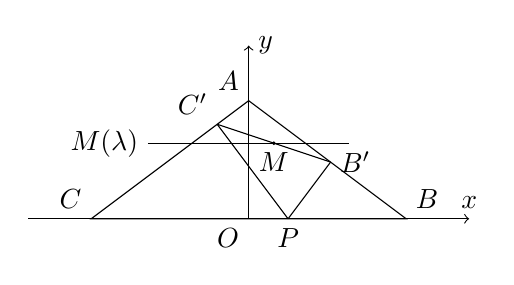
\begin{tikzpicture}[scale=1]
			          %projection ($(X)!(B')!(B)$)
			          %nommer chemin 'name path
			          %intersection \path [name intersections={of=d and gb,by=G}];
			          
			          %\draw[help lines] (-3,-3) grid (3,3);
			          \coordinate[label=below left:$O$](O) at (0,0);
			          \draw[->] (-2.8,0)--(2.8,0) node[above]{$x$};
				  \draw[->] (0,0)--(0,2.2) node[right]{$y$};
				  %TRIANGLE ABC
				  \coordinate[label=above left:$A$](A) at (0,1.5);
				  \coordinate[label=above right:$B$](B) at (2,0);
				  \coordinate[label=above left:$C$](C) at (-2,0);
				  \draw (A) -- (B) -- (C) -- cycle;				  
				  %P
				  \coordinate[label=below:$P$](P) at (0.5,0);
				  %B'C'
				  \coordinate[label=right:$B'$](B') at ($(A)!(P)!(B)$);
				  \coordinate[label=above left:$C'$](C') at ($(A)!(P)!(C)$);
				  \draw[visible on=<1>] (P) -- (B') (P) -- (C');
				  \draw[visible on=<2>] (B') -- node[below]{$M$} (C');
				  \fill[visible on=<2>] ($(B')!.5!(C')$) circle (0.025);
				  \draw[visible on=<2>] (-1.28,0.96) node[left]{$M(\lambda)$} -- (1.28,0.96);
				  \end{tikzpicture}
				  \end{figure}
				  \vspace{-1mm}
				  \begin{tcolorbox}[basic] 				      
				    \smallskip
				    \centering\underline{Procédé}
				     
				      \renewcommand{\theenumi}{\alph{enumi})}
				      \begin{enumerate}
					\item $B'\equiv BB' \bot B'P$, \\ \smallskip
					      $C'\equiv CC' \bot C'P$. \\[0.6em]
				      
					\item $M(\lambda)=\dfrac{B' + C'}{2}$,\\ \smallskip $\lambda \in[-b,b]$. \\[0.6em]
				    
					\item $d\equiv      \begin{cases} 
							    \bot\ B'C', \\
							    \ni P.
							    \end{cases}$ \\ \smallskip
							    + Point fixe.  
				      \end{enumerate}

				    
				    \end{tcolorbox}
		
		
		\column{.515\textwidth}\centering
		\underline{Résolution}\\ \flushleft
		$m_{AB} = -\dfrac{a}{b} \quad \rightarrow \quad m_{PB'}=\dfrac{b}{a}$. \\ \medskip
		\begin{align*}
		B'=&BB' \cap B'P= \begin{cases}
		                  y = -\frac{a}{b}x + a, \\
		                  y = \frac{b}{a}(x-\lambda).
		                  \end{cases} \\
		  =&(\ \frac{b(\lambda b+a^2)}{a^2 + b^2}\ ,\ \frac{a\ b(b-\lambda)}{a^2 + b^2}\ ).
		\end{align*} \smallskip
		
		
		De la même façon, \\ \medskip
		$C'=(\ \dfrac{b(\lambda b-a^2)}{a^2 + b^2}\ ,\ \dfrac{a\ b(b+\lambda)}{a^2 + b^2}\ )$. \\ \smallskip \hfill $\qed(a)$
		
		
		\onslide<+->
		\centering\noindent\rule{2cm}{0.4pt}\flushleft\vspace{-1mm}
		$M = (\dfrac{\lambda b^2}{a^2+b^2},\dfrac{a\ b^2}{a^2+b^2})$, $\lambda \in [-b,b]$. \\ \medskip
		$M(\lambda) \begin{cases}
		             x \in [-\dfrac{b^3}{a^2+b^2},\dfrac{b^3}{a^2+b^2}], \\
		             y = \dfrac{a\ b^2}{a^2+b^2}. 
		            \end{cases}\hspace{-4mm} \qed(b)$

		
		
		
		\end{columns}
    }
	
	\frame{ \onslide<+->
	  % résolution ex1
	      \begin{columns}[t]
		\column{.5\textwidth}\centering
				  \underline{Dessin}
				  \begin{figure}[h]
				  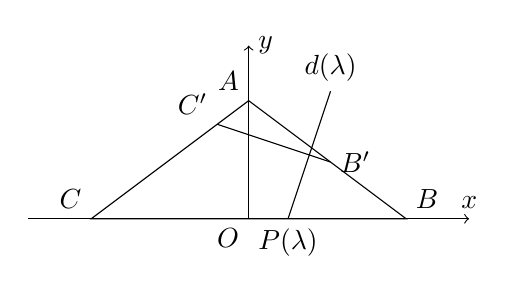
\begin{tikzpicture}[scale=1]
			          %projection ($(X)!(B')!(B)$)
			          %nommer chemin 'name path
			          %intersection \path [name intersections={of=d and gb,by=G}];
			          
			          %\draw[help lines] (-3,-3) grid (3,3);
			          \coordinate[label=below left:$O$](O) at (0,0);
			          \draw[->] (-2.8,0)--(2.8,0) node[above]{$x$};
				  \draw[->] (0,0)--(0,2.2) node[right]{$y$};
				  %TRIANGLE ABC
				  \coordinate[label=above left:$A$](A) at (0,1.5);
				  \coordinate[label=above right:$B$](B) at (2,0);
				  \coordinate[label=above left:$C$](C) at (-2,0);
				  \draw (A) -- (B) -- (C) -- cycle;				  
				  %P
				  \coordinate[label=below:$P(\lambda)$](P) at (0.5,0);
				  %B'C'
				  \coordinate[label=right:$B'$](B') at ($(A)!(P)!(B)$);
				  \coordinate[label=above left:$C'$](C') at ($(A)!(P)!(C)$);
				  \draw (B') -- (C');
				  \draw (P) -- +($2*(B')!(P)!(C')-2*(P)$) node[above]{$d(\lambda)$};
				  \end{tikzpicture}
				  \end{figure}
				  \vspace{-2mm}
				  \begin{tcolorbox}[basic] 				      
				    \smallskip
				    \centering\underline{Procédé}
				     
				      \renewcommand{\theenumi}{\alph{enumi})}
				      \begin{enumerate}
					\item $B'\equiv BB' \bot B'P$, \\ \smallskip
					      $C'\equiv CC' \bot C'P$. \\[0.6em]
				      
					\item $M(\lambda)=\dfrac{B' + C'}{2}$,\\ \smallskip $\lambda \in[-b,b]$. \\[0.6em]
				    
					\item $d\equiv      \begin{cases} 
							    \bot\ B'C', \\
							    \ni P.
							    \end{cases}$ \\ \smallskip
							    + Point fixe.  
				      \end{enumerate}

				    
				    \end{tcolorbox}
		
		
		\column{.5\textwidth}\flushleft
		De (a), \\ \smallskip
		$B'= (\ \dfrac{b(\lambda b+a^2)}{a^2 + b^2}\ ,\ \dfrac{a\ b(b-\lambda)}{a^2 + b^2}\ )$, \\ \medskip
		$C'= (\ \dfrac{b(\lambda b-a^2)}{a^2 + b^2}\ ,\ \dfrac{a\ b(b+\lambda)}{a^2 + b^2}\ )$. \\ \bigskip
		$m_{C'B'} = -\dfrac{\lambda}{a} \quad \rightarrow \quad m_{d}=\dfrac{a}{\lambda}$. \\ \bigskip
		
		$d \equiv \begin{cases}
		           y=\dfrac{a}{\lambda}(x-\lambda),& \lambda\neq 0. \\
		           x=0,& \lambda=0.
		          \end{cases}$ \\ \bigskip
		Le point fixe est $(0,-a)$. \hfill $\qed(c)$

		
		
		\end{columns}
    }
  
\end{document}
